% !TEX program = xelatex
% The No Paint Brushbook: every brush of nopaint.art (2021), A to Z, each with
% the game's own help and what a browser saw when it ran the brush.
% A sister to Aesthetic Spells (../arxiv-magicians-manual); both are set on the
% half-letter page in ../ac-booklet.sty.
%
% Generated parts (do not edit): entries.tex, tables.tex, tally.tex, shots/,
% cover.jpg. See gen-entries.mjs and notes.md.
\documentclass[10pt,twoside]{article}
\usepackage{../ac-booklet}
\usepackage{../ac-source-bundle}
\hypersetup{pdftitle={The No Paint Brushbook},pdfauthor={@jeffrey}}
% No Paint's own colours: the title's yellow and the prompt's green.
\definecolor{npyellow}{RGB}{255,221,0}
\definecolor{npgreen}{RGB}{0,80,0}
\definecolor{npink}{RGB}{24,24,32}

% One brush. #1 name, #2 options, #3 kind, #4 label, #5 who made it,
% #6 the game's sentence, #7 fields, #8 the strip, #9 what it started on.
\newlength{\stripwidth}
\newcommand{\brushentry}[9]{\par\addvspace{0.85em}\noindent\extramarks{#1}{#1}%
 \ifx\relax#5\relax\else\marginpar[\sideup\raggedleft\footnotesize\itshape\color{acdark}by #5]{\sideup\raggedright\footnotesize\itshape\color{acdark}by #5}\fi%
 \begin{minipage}[t]{\linewidth}\setlength{\parskip}{0pt}\setlength{\stripwidth}{0.72\linewidth}\phantomsection\label{#4}%
 {\large\spl{#1}}\ifx\relax#2\relax\else\ \textit{\small #2}\fi\hfill{\footnotesize\itshape #3}\par\vspace{0.12em}
 \noindent #6\par\vspace{0.2em}#7%
 \ifx\relax#8\relax\else\par\vspace{0.5em}\noindent\includegraphics[width=\stripwidth]{#8}\par\vspace{0.1em}%
 \noindent{\scriptsize\color{acgray}\makebox[0.370\stripwidth][l]{#9}\makebox[0.272\stripwidth][l]{the proposal}after Paint}\fi
 \end{minipage}\par}
\newcommand{\brushcount}{38}\newcommand{\tallyworks}{37}\newcommand{\tallydiffers}{0}\newcommand{\tallyuntested}{1}\newcommand{\paintercount}{18}\newcommand{\brushtablecount}{18}\newcommand{\filtertablecount}{17}\newcommand{\testdate}{November 18, 2026}


% Margin drawings: small pieces of the game's screen.
\newcommand{\vigbuttons}{\tikz{\fill[white] (0,0) rectangle (2.3,0.62);\draw[acgray,line width=0.4pt] (0,0) rectangle (2.3,0.62) (1.15,0) -- (1.15,0.62);
 \node[font=\sffamily\bfseries\footnotesize,text=npink] at (0.575,0.31) {No};\node[font=\sffamily\bfseries\footnotesize,text=npink] at (1.725,0.31) {Paint};}}
\newcommand{\vigprompt}{\tikz{\node[fill=npgreen,minimum width=2.3cm,minimum height=0.62cm,inner sep=2pt,font=\ttfamily\scriptsize,text=white]{Softy: 128 128 S ?};}}
\newcommand{\vigcode}{\tikz{\fill[acgray!25] (0,0) rectangle (2.3,0.62);\node[anchor=south east,font=\ttfamily\scriptsize,text=npink] at (2.24,0.04) {XXXXXXXX};}}

\begin{document}
% ====================== COVER ======================
\newgeometry{left=0.6in,right=0.6in,top=0.85in,bottom=0.7in}
\thispagestyle{empty}
\begin{center}
{\acbold\fontsize{31}{35}\selectfont\color{acdark} The No Paint Brushbook}\par
\vspace{0.7em}{\large\itshape\color{acdark} (every brush and filter of nopaint.art, with pictures)}\par
\vspace{1.6em}
\IfFileExists{cover.jpg}{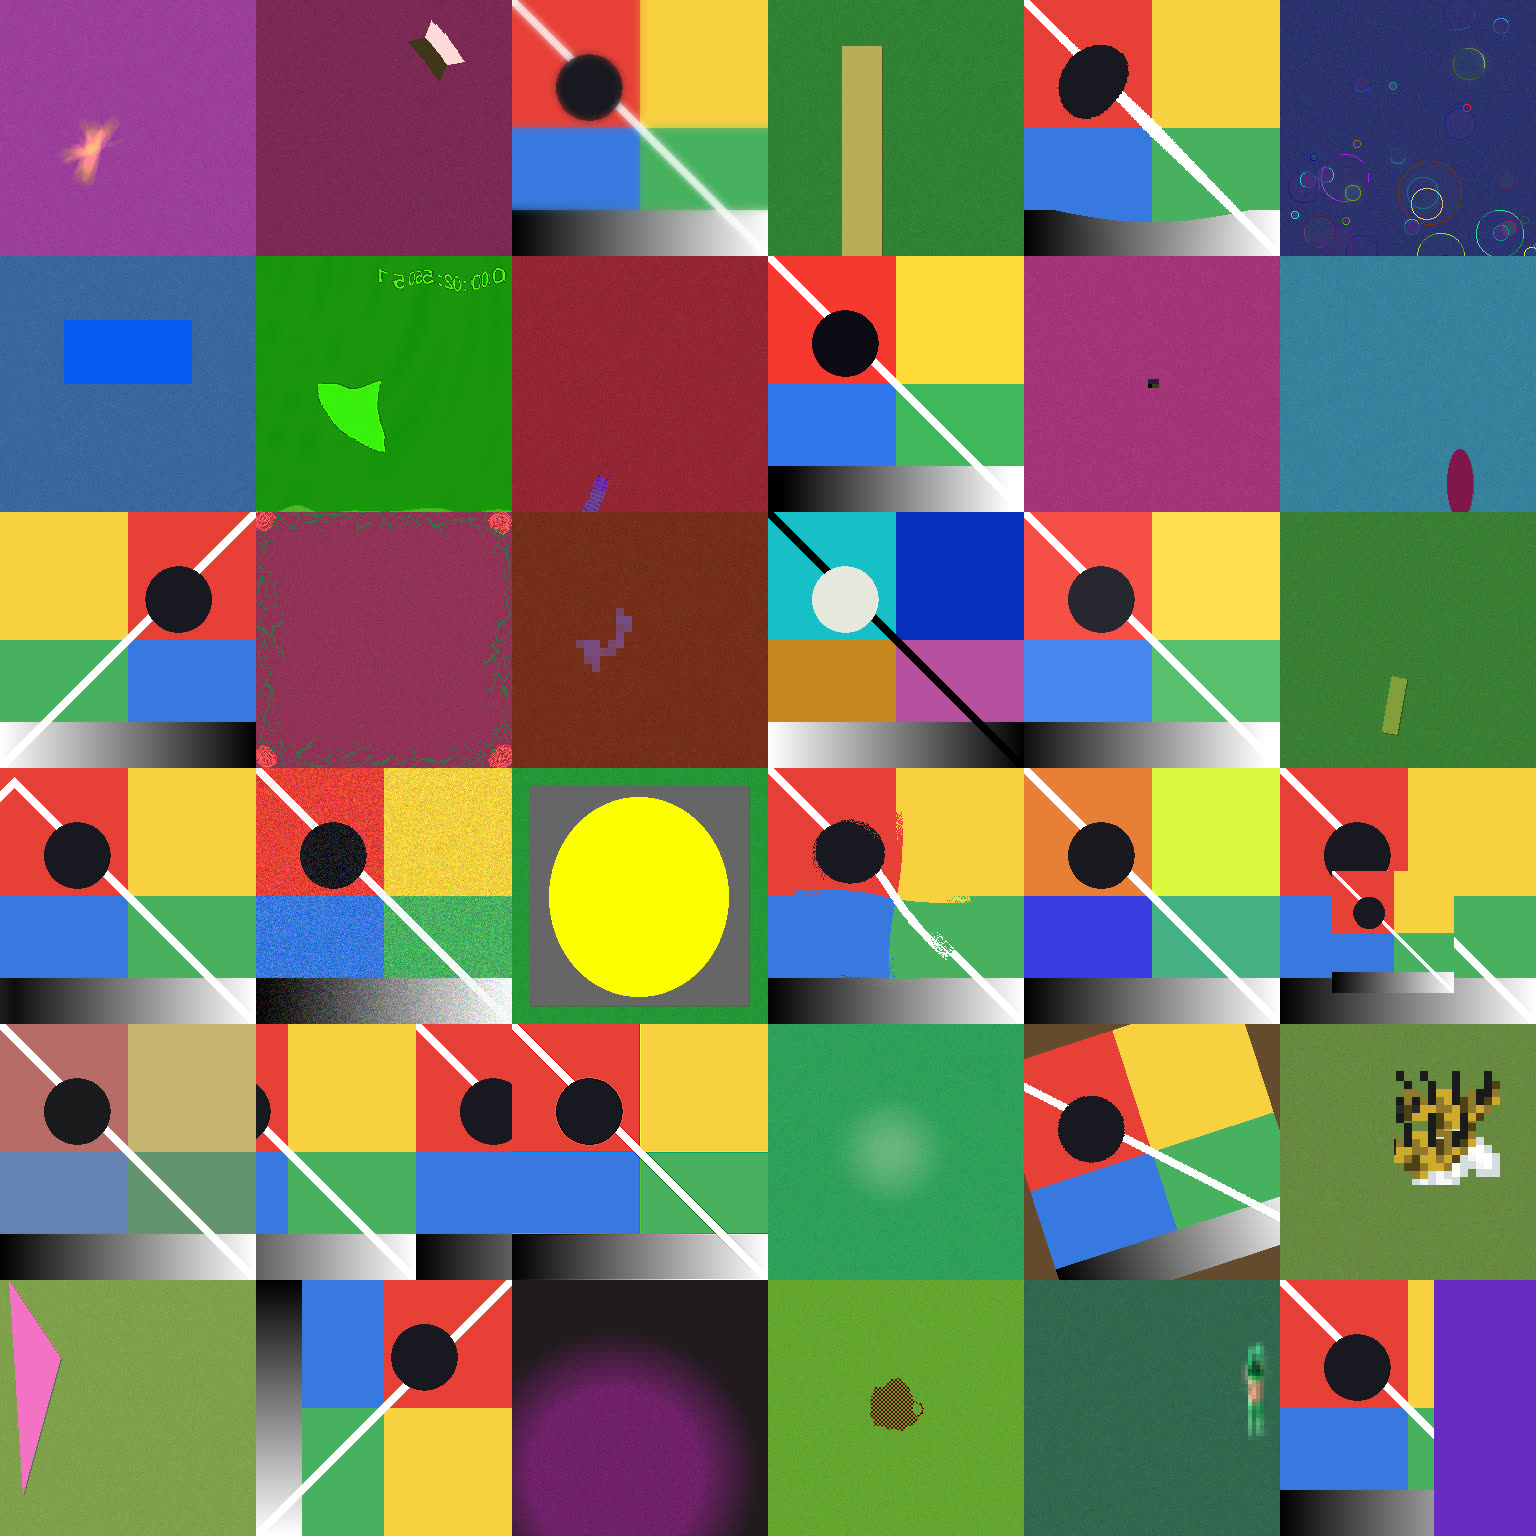
\includegraphics[width=0.86\linewidth]{cover.jpg}}{}\par
\vspace{0.7em}
{\footnotesize\sffamily\color{acdark} What each brush left behind when a browser pressed Paint, in the order of the book.}\par
\vfill
\begin{minipage}{0.8\linewidth}\centering\itshape\color{acdark}
Press ``Paint'' if you like what you see, or ``No'' if you don't.\par
\smallskip{\upshape\footnotesize\color{acgray} the game's own description, 2021}
\end{minipage}\par
\vfill
{\small\color{acgray} \href{https://prompt.ac/@jeffrey}{@jeffrey} · \ac{} · First edition, November 18, 2026}\par
\end{center}
\clearpage
\restoregeometry

% ====================== FRONT MATTER ======================
\thispagestyle{empty}
\vspace*{0.6em}
\noindent\textbf{Abstract.} No Paint is a painting game with two buttons. It shows you something it could do to your painting, and you answer No or Paint. It has been at \url{https://nopaint.art} since 2021 and people still paint with it. This book is the list of things it can do: \brushcount{} brushes from A to Z, each with the game's own words for it, the options it takes, how often the game offers it, and pictures of one run.

\vspace{0.7em}
\noindent\textbf{How to read it.} Words set like \spl{this} are typed at the game's prompt. Each entry shows three pictures: the painting before, the proposal on the screen, and the painting after Paint. A \emph{brush} adds something, so it starts on a new painting. A \emph{filter} changes what is there, so it starts on a test card. The label under the first picture says which.

\vspace{0.7em}
\noindent\textbf{Every entry has a line marked \textsc{ran}.} It says what a real browser saw on \testdate{} when it ran the brush twice, once answered Paint and once answered No. Of \brushcount{} brushes, \tallyworks{} did both as they should, \tallydiffers{} did something else and the entry says what, and \tallyuntested{} were not run.

\vspace{0.9em}
{\small\noindent\begin{tabularx}{\linewidth}{@{}L@{}r@{}}
How No Paint works & \pageref{ch:how} \\
The brushes, A to Z & \pageref{ch:brushes} \\
Tables & \pageref{ch:tables} \\
How this book was made & \pageref{ch:made} \\
\end{tabularx}}
\clearpage

% ====================== HOW IT WORKS ======================
\chapter{How No Paint works}\label{ch:how}
\sidevig{Two buttons.}{\vigbuttons}The game picks a brush and shows it at work on your painting. This is a \emph{proposal}. Nothing is kept yet. Press \emph{Paint} and what you see goes into the painting. Press \emph{No} and it is gone. Either way the next proposal comes at once.

\side{What it picks.}The game keeps two lists. One has \brushtablecount{} brushes, which add something: a box, a stamp, a worm. The other has \filtertablecount{} filters, which change what is already there: blur, flip, zoom. For each proposal it first picks a list, with even odds, and then picks from that list by weight. A heavy brush comes more often. \spl{Stamp} is the heaviest and \spl{Walker} the lightest. The tables at the back give every weight.

\sidevig{The prompt.}{\vigprompt}You can also ask for a brush. Tap the prompt and type its name exactly. The game's help says the rest: use a colon to add options, and keep an option random with a question mark. \spl{Softy: 128 128 S ?} is a small soft streak at the middle of the painting in a colour the game chooses. Type nothing, or \spl{?}, and the game picks for you.

\side{Options.}Most options are places, sizes and colours. A place is two numbers from 0 to 255, counted from the top left corner, because the painting is 256 dots wide and 256 tall. A colour is six letters and digits, from \spl{000000} (black) to \spl{FFFFFF} (white). Leave an option out and the game chooses it. The prompt then shows the choice in grey, and the \textsc{ran} lines in this book quote it.

\side{Three by name only.}\spl{Camera}, \spl{Load} and \spl{Playlist} are never proposed. \spl{Camera} shows your device's camera. \spl{Playlist} runs a written sequence of brushes: the game has six, and it can read one from a text file. \spl{Load} brings in a picture from your device or a painting by its code.

\sidevig{Codes.}{\vigcode}Save a painting and the game gives it a code of eight letters and digits, shown in the corner. \spl{Load} followed by a code brings that painting back, on any device.

\side{A new painting.}A new painting is not white. In every run of the test it began as one flat colour with a fine grain over it, a different colour each time. The \emph{before} pictures of the brushes show it.

\side{Who made it.}The page credits Jeffrey Alan Scudder with Alex Freundlich, Ella Fleck, Camille Klein and friends. The game's help names the maker of each brush, and \paintercount{} painters whose drawings \spl{Stamp} places. This book prints those names as the game does.

% ====================== THE BRUSHES ======================
\chapter{The brushes}\label{ch:brushes}
% Generated by gen-entries.mjs from brushes.json and e2e-summary.json. Do not edit by hand.

% A
\brushentry{Aura}{X Y}{brush}{br:1}{@erin}{%
A stain from a higher plane.}{%
\field{X, Y}{0 to 255}
\field{odds}{About 1.5 in 100 proposals.}
\field{ran}{Typed \spl{Aura}; it ran as \spl{Aura 93 150}. Paint changed the painting; No left it as it was.}}{shots/Aura.jpg}{a new painting}

% B
\brushentry{Banner}{X Y Angle}{brush}{br:2}{@alex}{%
Grab this freak flag and fly it too.}{%
\field{X, Y}{0 to 255}
\field{Angle}{0 to 360}
\field{odds}{About 3.6 in 100 proposals.}
\field{ran}{Typed \spl{Banner}; it ran as \spl{Banner 189 62 328}. Paint changed the painting; No left it as it was.}}{shots/Banner.jpg}{a new painting}
\brushentry{Blur}{}{filter}{br:3}{@jeffrey}{%
Bring everything out of focus, or cast a little glow.}{%
\field{odds}{About 2.9 in 100 proposals.}
\field{ran}{\spl{Blur}. Paint changed the painting; No left it as it was.}}{shots/Blur.jpg}{the test card}
\brushentry{Box}{X Y W H Color}{brush}{br:4}{@jeffrey}{%
Make a colored rectangle.}{%
\field{X, Y}{0 to 255}
\field{W, H}{1 to 255}
\field{Color}{000000 to FFFFFF}
\field{odds}{About 5.5 in 100 proposals.}
\field{ran}{Typed \spl{Box}; it ran as \spl{Box 94 172 40 251 5AADB9}. Paint changed the painting; No left it as it was.}}{shots/Box.jpg}{a new painting}
\brushentry{Breathe}{X Y Scale}{brush}{br:5}{@jeffrey}{%
Inflate the picture from behind.}{%
\field{X, Y}{0 to 255}
\field{Scale}{1 to 5}
\field{odds}{About 1.8 in 100 proposals.}
\field{ran}{\spl{Breathe 128 128 5}. Paint changed the painting; No left it as it was.}}{shots/Breathe.jpg}{the test card}
\brushentry{Bubbles}{}{brush}{br:6}{@erin}{%
Everyone loves them!}{%
\field{odds}{About 2.2 in 100 proposals.}
\field{ran}{\spl{Bubbles}. Paint changed the painting; No left it as it was.}}{shots/Bubbles.jpg}{a new painting}
\brushentry{Build}{X Y}{brush}{br:7}{@jeffrey}{%
Add some structure with square colored blocks.}{%
\field{X, Y}{0 to 255}
\field{odds}{About 3.6 in 100 proposals.}
\field{ran}{Typed \spl{Build}; it ran as \spl{Build 212 107}. Paint changed the painting; No left it as it was.}}{shots/Build.jpg}{a new painting}

% C
\brushentry{Camera}{Number FX}{by name}{br:8}{@jeffrey}{%
Show a LIVE feed from your device's camera.}{%
\field{Number}{1 to ?}
\field{FX}{1 to 10}
\field{on a phone}{\spl{Camera: Facing FX} Facing: Front or Back; FX: 1 to 10}
\field{odds}{Never proposed. It comes only when you type it.}
\field{ran}{Typed \spl{Camera}; it ran as \spl{Camera 1 10}. Paint changed the painting; No left it as it was.}}{shots/Camera.jpg}{a new painting}
\brushentry{Caterpillar}{Length}{brush}{br:9}{@erin}{%
A wandering little buggy.}{%
\field{Length}{3 to 32}
\field{odds}{About 0.9 in 100 proposals.}
\field{ran}{\spl{Caterpillar 32}. Paint changed the painting; No left it as it was.}}{shots/Caterpillar.jpg}{a new painting}
\brushentry{Contrast}{Amount}{filter}{br:10}{@jeffrey}{%
Color relationships grow closer together or further apart.}{%
\field{Amount}{More or Less}
\field{odds}{About 2.9 in 100 proposals.}
\field{ran}{Typed \spl{Contrast}; it ran as \spl{Contrast More}. Paint changed the painting; No left it as it was.}}{shots/Contrast.jpg}{the test card}

% D
\brushentry{Dark Window}{X Y}{brush}{br:11}{@jeffrey}{%
Keep it edgy and goth.}{%
\field{X, Y}{0 to 255}
\field{odds}{About 2.2 in 100 proposals.}
\field{ran}{\spl{Dark Window 128 128}. Paint changed the painting; No left it as it was.}}{shots/Dark-Window.jpg}{a new painting}

% E
\brushentry{Ellipse}{X Y W H C}{brush}{br:12}{@jeffrey}{%
Make a colored ellipse.}{%
\field{X, Y}{0 to 255}
\field{W, H}{3 to 255}
\field{C}{000000 to FFFFFF}
\field{odds}{About 2.9 in 100 proposals.}
\field{ran}{Typed \spl{Ellipse}; it ran as \spl{Ellipse 181 227 26 70 4C1780}. Paint changed the painting; No left it as it was.}}{shots/Ellipse.jpg}{a new painting}

% F
\brushentry{Flip}{Axis}{filter}{br:13}{@jeffrey}{%
Reflect the whole picture vertically or horizontally.}{%
\field{Axis}{H or V}
\field{odds}{About 2.9 in 100 proposals.}
\field{ran}{Typed \spl{Flip}; it ran as \spl{Flip H}. Paint changed the painting; No left it as it was.}}{shots/Flip.jpg}{the test card}
\brushentry{Frame}{}{brush}{br:14}{@camille}{%
Choose from a collection of bespoke frames for your painting.}{%
\field{odds}{About 0.9 in 100 proposals.}
\field{ran}{\spl{Frame}. Paint changed the painting; No left it as it was.}}{shots/Frame.jpg}{a new painting}

% G
\brushentry{Grid Worm}{X Y}{brush}{br:15}{@jeffrey}{%
A long bug that loves techno.}{%
\field{X, Y}{0 to 255}
\field{odds}{About 1.3 in 100 proposals.}
\field{ran}{Typed \spl{Grid Worm}; it ran as \spl{Grid Worm 119 125}. Paint changed the painting; No left it as it was.}}{shots/Grid-Worm.jpg}{a new painting}

% I
\brushentry{Invert}{}{filter}{br:16}{@jeffrey}{%
Turn the colors of your painting inside-out.}{%
\field{odds}{About 2.9 in 100 proposals.}
\field{ran}{\spl{Invert}. Paint changed the painting; No left it as it was.}}{shots/Invert.jpg}{the test card}

% L
\brushentry{Light Bump}{Amount}{filter}{br:17}{@jeffrey}{%
A tap from Heaven and a dusting of Hell.}{%
\field{Amount}{More or Less}
\field{odds}{About 2.9 in 100 proposals.}
\field{ran}{Typed \spl{Light Bump}; it ran as \spl{Light Bump More}. Paint changed the painting; No left it as it was.}}{shots/Light-Bump.jpg}{the test card}
\brushentry{Line}{X1 Y1 X2 Y2 W C}{brush}{br:18}{@jeffrey}{%
Make a colored line.}{%
\field{X?, Y?}{0 to 255}
\field{Width}{1 to 16}
\field{Color}{000000 to FFFFFF}
\field{odds}{About 2.9 in 100 proposals.}
\field{ran}{Typed \spl{Line}; it ran as \spl{Line 110 221 118 164 16 3C9E83}. Paint changed the painting; No left it as it was.}}{shots/Line.jpg}{a new painting}
\brushentry{Load}{Code}{by name}{br:19}{@jeffrey}{%
Import from your device or enter code from the corner of a painting.}{%
\field{Code}{XXXXXXXX}
\field{odds}{Never proposed. It comes only when you type it.}
\field{ran}{Not run: opens a file picker, or fetches a painting from the save server.}}{}{a new painting}

% M
\brushentry{Mirror}{Side}{filter}{br:20}{@alex}{%
Time to reflect \$.}{%
\field{Side}{Top, Bottom, Left, Right}
\field{odds}{About 2.9 in 100 proposals.}
\field{ran}{Typed \spl{Mirror}; it ran as \spl{Mirror Left}. Paint changed the painting; No left it as it was.}}{shots/Mirror.jpg}{the test card}

% N
\brushentry{Noise}{}{filter}{br:21}{@jeffrey}{%
It always helps me sleep.}{%
\field{odds}{About 2.9 in 100 proposals.}
\field{ran}{\spl{Noise}. Paint changed the painting; No left it as it was.}}{shots/Noise.jpg}{the test card}

% P
\brushentry{Playlist}{Name}{by name}{br:22}{@jeffrey}{%
Run a composed sequence or load your own from a .txt file.}{%
\field{Name}{Landscape, Frog Dies, Gift, Polka Dots, Well, Smiley}
\field{odds}{Never proposed. It comes only when you type it.}
\field{ran}{\spl{Playlist: Smiley}. Its first steps painted with no button pressed.}}{shots/Playlist.jpg}{a new painting}

% Q
\brushentry{Quicksand}{X Y Scale}{filter}{br:23}{@jeffrey}{%
Suck pixels into a granular spiral.}{%
\field{X, Y}{0 to 255}
\field{Scale}{1 to 4}
\field{odds}{About 2.9 in 100 proposals.}
\field{ran}{Typed \spl{Quicksand}; it ran as \spl{Quicksand 114 130 4}. Paint changed the painting; No left it as it was.}}{shots/Quicksand.jpg}{the test card}

% R
\brushentry{Rainbow}{}{filter}{br:24}{@jeffrey}{%
Cycle through a digital color wheel.}{%
\field{odds}{About 2.9 in 100 proposals.}
\field{ran}{\spl{Rainbow}. Paint changed the painting; No left it as it was.}}{shots/Rainbow.jpg}{the test card}
\brushentry{Recurse}{X Y}{filter}{br:25}{@ella}{%
Nest your composition inside itself.}{%
\field{X, Y}{0 to 255}
\field{odds}{About 2.9 in 100 proposals.}
\field{ran}{Typed \spl{Recurse}; it ran as \spl{Recurse 100 198}. Paint changed the painting; No left it as it was.}}{shots/Recurse.jpg}{the test card}

% S
\brushentry{Saturate}{Amount}{filter}{br:26}{@jeffrey}{%
Make those existing hues pop, or not!}{%
\field{Amount}{More or Less}
\field{odds}{About 2.9 in 100 proposals.}
\field{ran}{Typed \spl{Saturate}; it ran as \spl{Saturate Less}. Paint changed the painting; No left it as it was.}}{shots/Saturate.jpg}{the test card}
\brushentry{Scroll}{Way}{filter}{br:27}{@jeffrey}{%
Shift the composition vertically or horizontally.}{%
\field{Way}{Up, Down, Left, Right}
\field{odds}{About 2.9 in 100 proposals.}
\field{ran}{Typed \spl{Scroll}; it ran as \spl{Scroll Left}. Paint changed the painting; No left it as it was.}}{shots/Scroll.jpg}{the test card}
\brushentry{Sharpen}{}{filter}{br:28}{@jeffrey}{%
This should clear things up.}{%
\field{odds}{About 2.9 in 100 proposals.}
\field{ran}{\spl{Sharpen}. Paint changed the painting; No left it as it was.}}{shots/Sharpen.jpg}{the test card}
\brushentry{Softy}{X Y Size Color}{brush}{br:29}{@jeffrey}{%
A soft and friendly streak that almost always satisfies.}{%
\field{X, Y}{0 to 255}
\field{Size}{S, M, L}
\field{Color}{000000 to FFFFFF}
\field{odds}{About 5.5 in 100 proposals.}
\field{ran}{Typed \spl{Softy: 128 128 L ?}; it ran as \spl{Softy 128 128 L BDD9C9}. Paint changed the painting; No left it as it was.}}{shots/Softy.jpg}{a new painting}
\brushentry{Spin}{}{filter}{br:30}{@jeffrey}{%
Rotate the composition quickly, sometimes leaves a ghostly trail.}{%
\field{odds}{About 2.9 in 100 proposals.}
\field{ran}{\spl{Spin}. Paint changed the painting; No left it as it was.}}{shots/Spin.jpg}{the test card}
\brushentry{Stamp}{Art Num X Y Dir Scale Mirror}{brush}{br:31}{17 painters}{%
Place one drawing from a painter's set. Each painter's handle names a set; Num picks the drawing.}{%
\field{Art}{@name}
\field{Num}{1 to ?}
\field{X, Y}{0-255}
\field{Dir}{U, D, L, R}
\field{Scale}{1-2}
\field{Mirror}{Y, N}
\field{art}{@jeffrey, @ella, @alex, @artur, @camille, @julia, @adelaide, @sean, @niki, @wilson, @Ivokyuftaf6666, @jesserobertsullivan, @usuuunaa, @deojavani, @aaron, @bn, @chance}
\field{odds}{About 7.3 in 100 proposals.}
\field{ran}{Typed \spl{Stamp}; it ran as \spl{Stamp @aaron 1 167 103 D 2 Y}. Paint changed the painting; No left it as it was.}}{shots/Stamp.jpg}{a new painting}

% T
\brushentry{Triangle}{X1 Y1 X2 Y2 X3 Y3 Color}{brush}{br:32}{@jeffrey}{%
Make a colored triangle.}{%
\field{X?, Y?}{0 to 255}
\field{Color}{000000 to FFFFFF}
\field{odds}{About 2.9 in 100 proposals.}
\field{ran}{Typed \spl{Triangle}; it ran as \spl{Triangle 60 78 8 0 24 216 C572F4}. Paint changed the painting; No left it as it was.}}{shots/Triangle.jpg}{a new painting}
\brushentry{Turn}{}{filter}{br:33}{@jeffrey}{%
Rotate the composition by 90 degrees.}{%
\field{odds}{About 2.9 in 100 proposals.}
\field{ran}{\spl{Turn}. Paint changed the painting; No left it as it was.}}{shots/Turn.jpg}{the test card}

% V
\brushentry{Vignette}{X Y Scale}{brush}{br:34}{1 painters}{%
}{%
\field{X, Y}{0 to 255}
\field{Scale}{1 to 5}
\field{art}{@adelaide}
\field{odds}{About 1.5 in 100 proposals.}
\field{ran}{Typed \spl{Vignette}; it ran as \spl{Vignette 97 190 5}. Paint changed the painting; No left it as it was.}}{shots/Vignette.jpg}{a new painting}

% W
\brushentry{Wafer}{X Y}{brush}{br:35}{@ella}{%
Patterned snack in several hues and sizes. Yum.}{%
\field{X, Y}{0 to 255}
\field{odds}{About 2.9 in 100 proposals.}
\field{ran}{\spl{Wafer 128 128}. Paint changed the painting; No left it as it was.}}{shots/Wafer.jpg}{a new painting}
\brushentry{Walker}{}{brush}{br:36}{@ella}{%
Ella goes on a walk!}{%
\field{odds}{About 0.7 in 100 proposals.}
\field{ran}{\spl{Walker}. Paint changed the painting; No left it as it was.}}{shots/Walker.jpg}{a new painting}
\brushentry{Wipe}{From}{filter}{br:37}{@jeffrey}{%
A field of color advances and retreats in cardinal directions:}{%
\field{From}{N, S, W, E NW, NE, SW, SE}
\field{odds}{About 2.9 in 100 proposals.}
\field{ran}{Typed \spl{Wipe}; it ran as \spl{Wipe E}. Paint changed the painting; No left it as it was.}}{shots/Wipe.jpg}{the test card}

% Z
\brushentry{Zoom}{X Y}{filter}{br:38}{@jeffrey}{%
Reframe the painting by moving in and out at an anchored position.}{%
\field{X, Y}{0 to 255}
\field{odds}{About 2.9 in 100 proposals.}
\field{ran}{Typed \spl{Zoom}; it ran as \spl{Zoom 173 143}. Paint changed the painting; No left it as it was.}}{shots/Zoom.jpg}{the test card}


% ====================== TABLES ======================
\chapter{Tables}\label{ch:tables}
\extramarks{}{}\noindent{\small \emph{Weight} is the number the game holds for the brush. \emph{In 100} is how many of 100 proposals it should be, counting the even pick between the two lists.}
% Generated by gen-entries.mjs. Do not edit by hand.
\backhead{Brushes: they add something}
\noindent{\footnotesize\begin{tabularx}{\linewidth}{@{}L r r r@{}}\toprule
 & weight & in 100 & page \\\midrule
\spl{Stamp} & 2 & 7.3 & \pageref{br:31} \\
\spl{Box} & 1.5 & 5.5 & \pageref{br:4} \\
\spl{Softy} & 1.5 & 5.5 & \pageref{br:29} \\
\spl{Banner} & 1 & 3.6 & \pageref{br:2} \\
\spl{Build} & 1 & 3.6 & \pageref{br:7} \\
\spl{Ellipse} & 0.8 & 2.9 & \pageref{br:12} \\
\spl{Line} & 0.8 & 2.9 & \pageref{br:18} \\
\spl{Triangle} & 0.8 & 2.9 & \pageref{br:32} \\
\spl{Wafer} & 0.8 & 2.9 & \pageref{br:35} \\
\spl{Bubbles} & 0.6 & 2.2 & \pageref{br:6} \\
\spl{Dark Window} & 0.6 & 2.2 & \pageref{br:11} \\
\spl{Breathe} & 0.5 & 1.8 & \pageref{br:5} \\
\spl{Aura} & 0.4 & 1.5 & \pageref{br:1} \\
\spl{Vignette} & 0.4 & 1.5 & \pageref{br:34} \\
\spl{Grid Worm} & 0.35 & 1.3 & \pageref{br:15} \\
\spl{Caterpillar} & 0.25 & 0.9 & \pageref{br:9} \\
\spl{Frame} & 0.25 & 0.9 & \pageref{br:14} \\
\spl{Walker} & 0.2 & 0.7 & \pageref{br:36} \\
\midrule total & 13.75 & 50 & \\\bottomrule
\end{tabularx}}
\backhead{Filters: they change what is there}
\noindent{\footnotesize\begin{tabularx}{\linewidth}{@{}L r r r@{}}\toprule
 & weight & in 100 & page \\\midrule
\spl{Blur} & 1 & 2.9 & \pageref{br:3} \\
\spl{Contrast} & 1 & 2.9 & \pageref{br:10} \\
\spl{Flip} & 1 & 2.9 & \pageref{br:13} \\
\spl{Invert} & 1 & 2.9 & \pageref{br:16} \\
\spl{Light Bump} & 1 & 2.9 & \pageref{br:17} \\
\spl{Mirror} & 1 & 2.9 & \pageref{br:20} \\
\spl{Noise} & 1 & 2.9 & \pageref{br:21} \\
\spl{Quicksand} & 1 & 2.9 & \pageref{br:23} \\
\spl{Rainbow} & 1 & 2.9 & \pageref{br:24} \\
\spl{Recurse} & 1 & 2.9 & \pageref{br:25} \\
\spl{Saturate} & 1 & 2.9 & \pageref{br:26} \\
\spl{Scroll} & 1 & 2.9 & \pageref{br:27} \\
\spl{Sharpen} & 1 & 2.9 & \pageref{br:28} \\
\spl{Spin} & 1 & 2.9 & \pageref{br:30} \\
\spl{Turn} & 1 & 2.9 & \pageref{br:33} \\
\spl{Wipe} & 1 & 2.9 & \pageref{br:37} \\
\spl{Zoom} & 1 & 2.9 & \pageref{br:38} \\
\midrule total & 17 & 50 & \\\bottomrule
\end{tabularx}}
\backhead{By name only}
\noindent{\footnotesize \spl{Camera} (p.\,\pageref{br:8}), \spl{Load} (p.\,\pageref{br:19}), \spl{Playlist} (p.\,\pageref{br:22}).}
\backhead{Who made which brush}
\noindent{\footnotesize\begin{tabularx}{\linewidth}{@{}l L@{}}\toprule
@jeffrey & \spl{Blur}, \spl{Box}, \spl{Breathe}, \spl{Build}, \spl{Camera}, \spl{Contrast}, \spl{Dark Window}, \spl{Ellipse}, \spl{Flip}, \spl{Grid Worm}, \spl{Invert}, \spl{Light Bump}, \spl{Line}, \spl{Load}, \spl{Noise}, \spl{Playlist}, \spl{Quicksand}, \spl{Rainbow}, \spl{Saturate}, \spl{Scroll}, \spl{Sharpen}, \spl{Softy}, \spl{Spin}, \spl{Triangle}, \spl{Turn}, \spl{Wipe}, \spl{Zoom} \\
@ella & \spl{Recurse}, \spl{Wafer}, \spl{Walker} \\
@erin & \spl{Aura}, \spl{Bubbles}, \spl{Caterpillar} \\
@alex & \spl{Banner}, \spl{Mirror} \\
@camille & \spl{Frame} \\
\bottomrule\end{tabularx}}


% ====================== HOW THIS BOOK WAS MADE ======================
\chapter{How this book was made}\label{ch:made}
\side{The words.}The sentence under each name, the option names and their ranges are the game's own help pages, read out of the 2021 project file by a script and printed without change. Two things are the book's: the sentence for \spl{Stamp}, which has none in the game, and the \textsc{odds} lines, worked out from the game's two weighted lists.

\side{The pictures.}A test ran the game in a browser with nobody watching (headless Chrome on a Mac mini). The build was the one served at nopaint.art, with one small script added so the test can type at the prompt, press the buttons and read the painting. For each brush it opened a new game, typed the name, waited 2.6 seconds, took the picture of the proposal, and pressed Paint. Then it did the same again and pressed No. Most names were typed with no options, so the game chose them. Six were typed with options, to put the mark at the middle or make it large enough to see; their \textsc{ran} lines show what was typed. Three slow brushes were watched for six to nine seconds. \spl{Breathe} started on the test card, because it needs something to inflate. The game was served from a folder and could reach nothing else, so no visit was counted and no painting was saved.

\side{What a pass means.}After Paint the painting must be different. After No it must be the same. The test does not judge whether the picture is the right one. A person looked at every strip in this book for that.

\side{Not shown.}Sound, and motion: many brushes move, and a strip shows one moment. The camera in the test was a stand-in, not a room. \spl{Load} was not run, because it opens a file picker or fetches a saved painting.

\side{Sources.}The game at \url{https://nopaint.art}. Its project file, kept by its makers. The test, \texttt{tests/browser/brushbook.e2e.mjs}, and the scripts beside this book, in the \ac{} repository.
\end{document}
